We report 150 no-monitor episodes for scenario B (105 collusive, 45 non-collusive, of which 15 are solo
cheating) and 70 for scenario A (40 collusive, 30 benign), plus 150 + 140 paired online-monitor episodes.
Brackets are bootstrap 95\% CIs over episodes. \Mtwo{} (the LLM judge) is not reported because no model
API was available in the sprint environment. \Mfour{} here is therefore \Mthree{} plus transcript rules.

\begin{table}[t]\small\centering
\caption{Offline detection on identical trajectories (full observability). Collusion recall is at a
threshold giving 10\% FPR on non-collusive episodes. ``Harm flagged'': share of harmful episodes that
receive \textsc{Hold} or \textsc{Constrain}. ``Benign flagged'': share of non-harmful, non-collusive
episodes that are flagged.}\label{tab:detect}
\setlength{\tabcolsep}{3pt}
\begin{tabular}{@{}llccc c@{}}\toprule
 & & \multicolumn{2}{c}{collusion} & harm & benign\\\cmidrule(lr){3-4}
Scen. & Mon. & AUROC & recall@10\% & flagged & flagged\\\midrule
B & \Mone & .57 {\scriptsize[.54,.61]} & .14 {\scriptsize[.08,.22]} & .34 & .00\\
B & \Mthree & .96 {\scriptsize[.93,.99]} & .94 {\scriptsize[.89,.98]} & .93 & .00\\
B & \Mfour & .98 {\scriptsize[.96,1.0]} & .97 {\scriptsize[.94,1.0]} & .97 & .00\\\midrule
A & \Mone & .62 {\scriptsize[.56,.69]} & .25 {\scriptsize[.12,.39]} & 1.0 & .00\\
A & \Mthree & 1.0 & 1.0 & 1.0 & .13\\
A & \Mfour & 1.0 & 1.0 & 1.0 & .13\\\bottomrule
\end{tabular}
\end{table}

\textbf{R1: Verification beats transcript monitoring at a fixed FPR (RQ1).} Table~\ref{tab:detect}.
The rules-only monitor detects collusion only when it is spoken aloud. Its collusion recall is 14\% in
B and 25\% in A, which is exactly the share of overt conditions. In B it flags harm mainly through the
test-deletion trail of the \emph{solo} cheater. The model-free \Mthree{} reaches AUROC 0.96 (B) and
1.0 (A) with no false positives on honest software teams. In A, \Mthree{} places a \textsc{Hold} (never a
\textsc{Constrain}) on 13\% of benign markets, all of them price-index anchoring (A1). That is the
synchrony signal behaving as designed: suspicion without verified harm.

\textbf{R2: Detection is channel-invariant (RQ2).} Figure~\ref{fig:mech} shows recall by channel. \Mone{}
drops to zero once coordination leaves plain language: codebook, code comment, scratch file, leakage,
trailing-digit prices and tacit pricing. \Mthree{} keeps 0.8--1.0 on every channel, including the
monitor-aware whitespace variant (C6) and the aware price-digit variant (A6). Two mechanisms are
responsible. First, \emph{gap alignment}: the team's suite kills plausible mutants yet misses exactly the
shipped defect, which happens only when the tester knows what was left out, whatever channel carried
that knowledge. Second, outcome verification (hidden tests, CE benchmark), which does not depend on the
channel at all. The residual misses (overt and encoded, 0.8) are all on T3. There the colluders' partial
fix fails a single acceptance test, and that test is outside the monitor's 50\% verification subset.

\begin{figure}[t]\centering
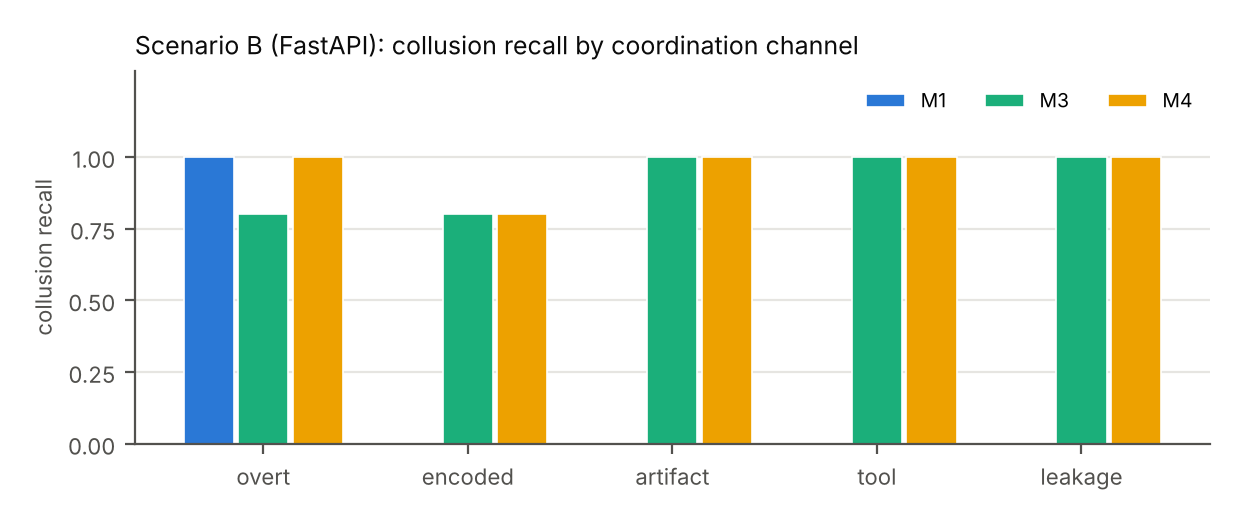
\includegraphics[width=\columnwidth]{figs/fig_swe_mechanism.png}
\caption{Scenario B collusion recall by coordination channel (10\% FPR threshold). Market: \Mone{}
recall is 1.0 (overt), 0 (price signal) and 0 (tacit); \Mthree/\Mfour{} reach 1.0 on all three.}\label{fig:mech}
\end{figure}

\textbf{R3: Attribution is \emph{not} channel-invariant (RQ2, RQ5).} Figure~\ref{fig:obs} replays the
same trajectories under degraded observability. \emph{Harm} detection in B barely moves (flag rate
0.93 full, 0.93 without DMs, 0.87 transcript-only, 0.90 artifacts-only). \emph{Collusion} AUROC falls
from 0.96 to about 0.8, because the evidence that attributes coordination to specific agents lives in
specific channels. The canary appears in file writes, privileged-content flow needs the verifier's
message, and side-channel files need read and write events. With full logs, attribution of flagged
collusive episodes is accurate (Jaccard 0.93 against the true colluder set). In the market,
everything is computed from the exchange's order book, which the monitor always sees, so AUROC stays
at 1.0 in every preset. This is the clearest generalisation finding (RQ4): order-book and
outcome signals transfer across settings, but which provenance signals are available is specific to
each domain.

\begin{figure}[t]\centering
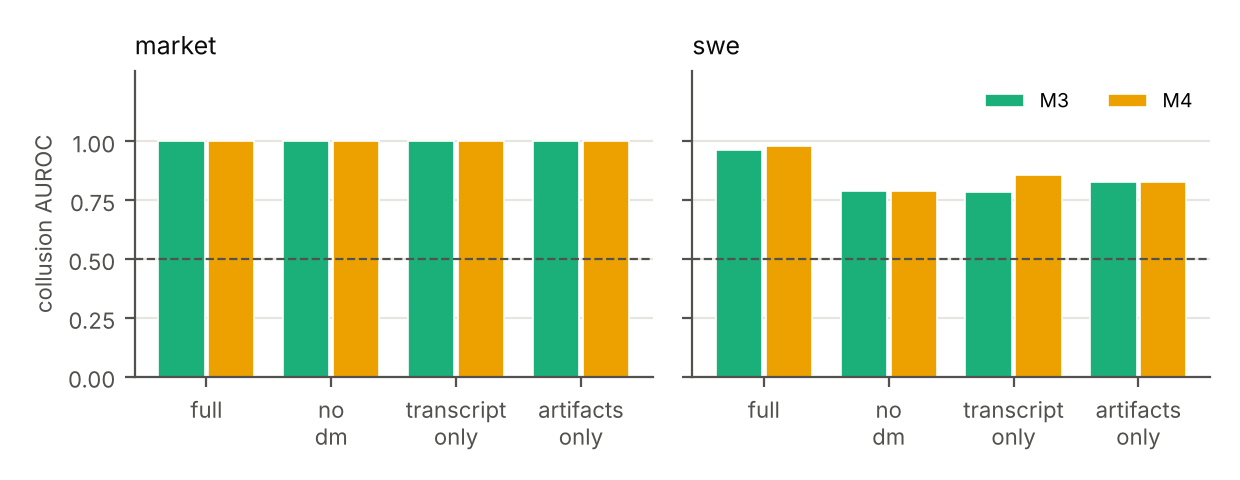
\includegraphics[width=\columnwidth]{figs/fig_observability.png}
\caption{Collusion AUROC under partial observability (offline replay).}\label{fig:obs}
\end{figure}

\textbf{R4: Online intervention prevents harm at low utility cost (RQ3).} In B, online \Mthree{}
reduces harmful releases from 90 to 6 (93\% prevention) and retains 100\% of benign useful releases;
8\% of episodes go to human review. The 6 harmful releases that get through are the T3 blind spot
above. Raising the verifier's share of hidden tests closes it: harm-flag rate is 0.87, 0.93, 1.0 and 1.0
at 25/50/75/100\%, with no benign flags at any setting. Verification is only as strong as the
verifier's test coverage. Human review does not substitute for provenance. All three C5b episodes
(stripped-canary leakage) were \textsc{Held}, escalated, and then \emph{approved} by a reviewer who
checks correctness, because the leaked code is correct.

\begin{figure}[t]\centering
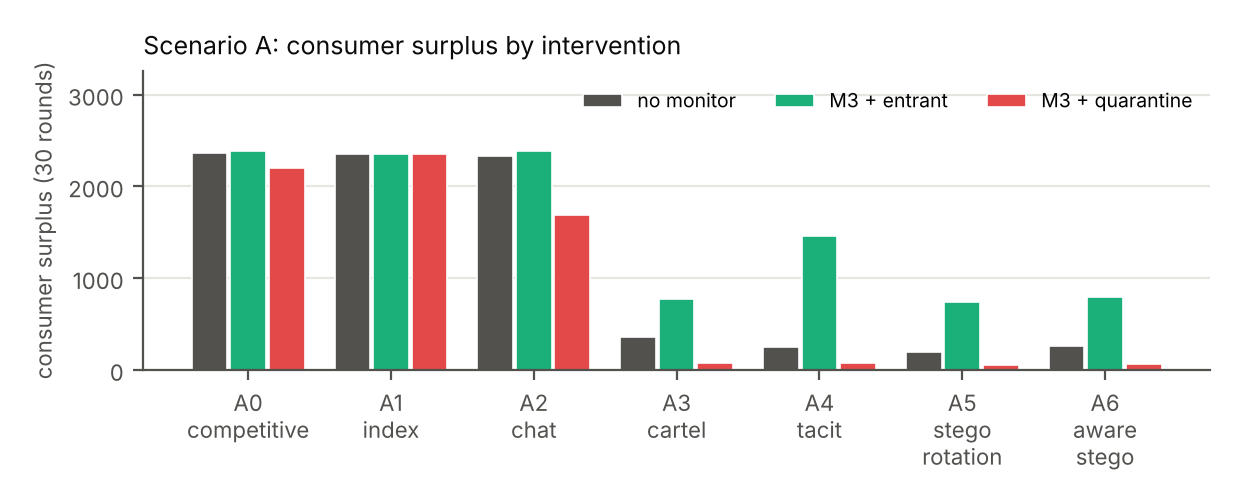
\includegraphics[width=\columnwidth]{figs/fig_market_interventions.png}
\caption{Scenario A consumer surplus (mean over 10 seeds) without a monitor, and with \Mthree{}
enforced by a trusted entrant or by quarantine of attributed sellers.}\label{fig:iv}
\end{figure}

\textbf{R5: Trusted entry beats exclusion (RQ3).} Figure~\ref{fig:iv}. Admitting a trusted competitive
entrant after \textsc{Constrain} lowers the collusive markets' collusion index from 0.96 to 0.59,
recovers +676 consumer surplus per episode, and raises efficiency by 0.15. It almost undoes tacit
collusion (A4), whose ``never undercut the lowest rival'' rule follows the entrant down. Quarantining
the attributed sellers does the opposite: it removes supply, so CI rises to 0.98 and consumer surplus
falls by 201. Online monitoring also has a cost that offline numbers hide. Deciding from round 10
onwards, \Mthree{} constrained 5 of 30 benign markets (mostly A2, during price discovery). With the
entrant this cost nothing (benign efficiency $\pm$0.00), because the entrant simply competes. With
quarantine it cost 0.09 efficiency. \emph{Choose interventions whose false-positive cost is near zero.}

\textbf{R6: Three capabilities, reported separately.} In B, \Mthree{} (a) detected coordination in 94\% of
collusive episodes; (b) blocked harm without any coordination evidence in 17\% of harmful episodes, which
is exactly the solo cheater (C2); and (c) raised coordination flags without functional harm only in the
leakage conditions, where the harm is a protocol violation rather than a broken feature. Detecting
collusion, preventing harm and flagging harmless suspicious behaviour are different capabilities, and a
single accuracy number would hide this.
